\chapter{Espacios métricos}
\begin{definition}[Espacio métrico]
Un \textbf{espacio métrico} es un par $\displaystyle \left(X, d\right) $ donde $\displaystyle X $ es un conjunto no vacío y $\displaystyle d : X \times X \to \R $ es una función que se llama \textbf{distancia} o \textbf{métrica}, tal que:
\begin{enumerate}
\item $\displaystyle d\left(x,y\right) \geq 0 $, $\displaystyle \forall x,y \in X $.
\item $\displaystyle d\left(x,y\right) = 0 \iff x = y $.
\item $\displaystyle d\left(x,y\right) = d\left(y,x\right) $, $\displaystyle \forall x,y \in X $.
\item (Propiedad triangular) $\displaystyle d\left(x,y\right) \leq d\left(x,z\right) + d\left(z,y\right) $, $\displaystyle \forall x,y,z \in X $.
\end{enumerate}
\end{definition}
\begin{eg} Algunos ejemplos de espacios métricos son:
\begin{enumerate}
\item Consideremos $\displaystyle \left(\R, d\right) $ donde $\displaystyle d\left(x,y\right) = \left|x - y\right| $.
\item La distancia euclídea en $\displaystyle \R^{2} = \left\{ \left(x,y\right) \; : \; x,y \in \R\right\} $: 
	\[ d\left(\left(x_{1}, x_{2}\right), \left(y_{1}, y_{2}\right)\right) = \sqrt{\left(x_{1}-y_{1}\right)^{2}+\left(x_{2}-y_{2}\right)^{2}}.\]
\item La 'métrica del taxi' en $\displaystyle \R^{2} $ con distancia:
	\[d _{1}\left(\left(x_{1}, x_{2}\right), \left(y_{1}, y_{2}\right)\right) = \left|x_{1} - y_{1}\right| + \left|x_{2}-y_{2}\right| .\]
\item Distancias geodésicas: el camino más corto (por ejemplo, en una superficie esférica el camino más corto entre dos puntos es un arco de circunferencia).
\item Distancias en $\displaystyle \R^{n} $. Si $\displaystyle x = \left(x_{1}, \ldots, x_{n}\right) $ e $\displaystyle y= \left(y_{1}, \ldots, y_{n}\right) $, consideramos la distancia euclídea
	\[d _{2}\left(x,y\right) = \sqrt{\left(x_{1}-y_{1}\right)^{2} + \cdots + \left(x_{n}-y_{n}\right)^{2}} .\]
También podemos generalizar la 'métrica del taxi':
\[ d _{1}\left(x,y\right) = \left|x_{1}-y_{1}\right| + \cdots + \left|x_{n}-y_{n}\right| .\]
También se puede considerar la métrica
\[d _{\infty}\left(x,y\right) = \max \left\{  \left|x_{i}-y_{i}\right| \; : \; 1 \leq i \leq n\right\}  .\]
\end{enumerate}
\end{eg}
\begin{definition}[Espacio discreto]
Sea $\displaystyle X \neq \emptyset $ un conjunto cualquiera, y definimos $\displaystyle \forall x,y \in X $ 
\[d\left(x,y\right) = 
\begin{cases}
0, \; \text{si} \; x = y \\
1, \; \text{si} \; x \neq y
\end{cases}
.\]
Se dice que $\displaystyle d $ es la \textbf{métrica discrecta} y $\displaystyle \left(X, d\right) $ el \textbf{espacio métrico discreto}.
\end{definition}
\begin{definition}[Subespacio métrico]
Sea $\displaystyle \left(X, d\right) $ un espacio métrico y sea $\displaystyle Y \subset X $. Se define la \textbf{métrica relativa} (o \textbf{restringida}) a $\displaystyle Y $ como $\displaystyle d _{Y}\left(y, y'\right)  = d\left(y, y'\right) $, $\displaystyle \forall y, y' \in Y $. Entonces, $\displaystyle \left(Y, d _{Y}\right) $ es un espacio métrico que llamaremos \textbf{subespacio} de $\displaystyle X $.
\end{definition}
\section{Espacios normados}
\begin{definition}[Espacio normado]
Un \textbf{espacio normado} es un par $\displaystyle \left(E, \left\| \cdot \right\|\right) $ donde $\displaystyle E $ es un espacio vectorial y $\displaystyle \| \cdot \| : E \to \R $ es una función que se llama \textbf{norma} tal que:
\begin{enumerate}
\item $\displaystyle \| x \| \geq 0 $, $\displaystyle \forall x \in E $.
\item $\displaystyle \| x \| = 0 \iff x = 0 $.
\item $\displaystyle \| \lambda x \| = \left|\lambda \right|\|x\| $, $\displaystyle \forall \lambda \in \K, \forall x \in E $ \footnote{En este curso $\displaystyle \K $ va a ser principalmente $\displaystyle \R $.}.
\item $\displaystyle \| x + y \| \leq \| x \| + \| y \|$, $\displaystyle \forall x,y \in E $.
\end{enumerate}
\end{definition}
\begin{prop}
Sea $\displaystyle \left(E, \| \cdot \|\right) $ un espacio normado. Si definimos 
\[d\left(x,y\right) = \| x- y\|, \forall x,y \in E ,\]
se obtene que $\displaystyle d $ es una distancia en $\displaystyle E $, que se llama \textbf{asociada} a la norma. 
\end{prop}
\begin{proof}
Demostremos todas las propiedades de las métricas:
\begin{enumerate}
\item Tenemos que $\displaystyle d\left(x,y\right) = \|x-y\| \geq 0 $, $\displaystyle \forall x,y \in E $.
\item $\displaystyle d\left(x,y\right) = 0 \iff \|x-y\|=0\iff x - y = 0 \iff x = y $.
\item $\displaystyle d\left(x,y\right) = \|y - x\| = \left|-1\right| \|x-y\| = \|x-y\| = d\left(x,y\right) $.
\item $\displaystyle d\left(x,y\right) = \| x- y\| = \|x-z + z- y\| \leq \|x - z\| + \|z - y\| = d\left(x,z\right) + d\left(z,y\right) $.
\end{enumerate}
\end{proof}
\begin{observation}
En $\displaystyle \R^{n} $, dado $\displaystyle x = \left(x_{1}, \ldots, x_{n}\right) \in \R^{n} $ se definen:
\[ \text{(Norma euclídea)} \quad \|x\|_{2} = \sqrt{x^{2}_{1} + \cdots + x^{2}_{n}} .\]
\[\|x\|_{1} = \left|x_{1}\right| + \cdots + \left|x_{n}\right| .\]
\[ \|x\|_{\infty} = \max \left\{ \left|x_{i}\right| \; : \; 1 \leq i \leq n\right\}  .\]
\end{observation}
\begin{prop}[Relación entre las normas en $\displaystyle \R^n $]
$\displaystyle \forall x = \left(x_{1}, \ldots, x_{n}\right) \in \R^{n} $, 
\[ \|x\| _{\infty} \leq \|x\|_{2} \leq \|x\|_{1} \leq n\|x\|_{\infty} .\]
\end{prop}
\begin{proof}
Supongamos que $\displaystyle \left|x_{i_{0}}\right| = \|x\|_{\infty} $. Entonces, tenemos que
\[ \displaystyle \left|x_{i_{0}}\right|^{2} \leq \left|x_{1}\right|^{2} + \cdots + \left|x_{n}\right|^{2}.\]
Dado que la función de la raíz es creciente, tenemos que 
\[ \|x\|_{\infty} = \left|x_{i_{0}}\right| \leq \sqrt{\left|x_{1}\right|^{2} + \cdots + \left|x_{n}\right|^{2}} = \|x\|_{2}.\]
Por otro lado, tenemos que
\[ \|x\|_{1}^{2} = \left(\left|x_{1}\right| + \cdots + \left|x_{n}\right|\right)^{2}= \left|x_{1}\right|^{2} + \cdots + \left|x_{n}\right|^{2} + C \footnote{ $\displaystyle C \geq 0. $}  \geq \left|x_{1}\right|^{2} + \cdots + \left|x_{n}\right|^{2} = \|x\|_{2}^{2} .\]
Finalmente, tenemos que 
\[ \|x\|_{1} = \left|x_{1}\right| + \cdots + \left|x_{n}\right| \leq \left|x_{i_{0}}\right| + \cdots + \left|x_{i_{0}}\right| = n \left|x_{i_{0}}\right| = n \|x\|_{\infty} .\]
\end{proof}
\begin{definition}
Dos normas $\displaystyle \| \cdot \| $ y $\displaystyle \| \cdot \|' $ en un mismo espacio vectorial $\displaystyle E $ son \textbf{equivalentes} cuando existen $\displaystyle m, M > 0 $ tales que 
\[m \|x\|' \leq \|x\| \leq M \|x\|', \; \forall x \in E .\]
\end{definition}
\begin{observation}
Hemos visto en la proposición anterior que $\displaystyle \| \cdot\|_{1}, \| \cdot \|_{2} $ y $\displaystyle \| \cdot \|_{\infty} $ son equivalentes en $\displaystyle \R^{n} $.
\end{observation}
\begin{definition}[Producto escalar]
Sea $\displaystyle E $ un espacio vectorial real. Un \textbf{producto escalar} en $\displaystyle E $ es una forma bilineal, simétrica y definida positiva. Es decir, una aplicación $\displaystyle \left\langle ,  \right\rangle : E \times E \to \R $ tal que 
\begin{enumerate}
\item $\displaystyle \left\langle \lambda x + \mu y, z \right\rangle = \lambda \left\langle x, z \right\rangle +\mu \left\langle y, z \right\rangle  $, $\displaystyle \forall x,y,z \in E, \forall \lambda, \mu \in \R $. 
\item $\displaystyle \left\langle x, y \right\rangle = \left\langle y, x \right\rangle  $, $\displaystyle \forall x,y \in E $.
\item $\displaystyle \forall x\in E $, $\displaystyle \left\langle x, x \right\rangle \geq 0 $ y $\displaystyle \left\langle x, x \right\rangle = 0 \iff x = 0 $.
\end{enumerate}
\end{definition}
\begin{observation}
En este caso, denotaremos $\displaystyle \|x\| = \sqrt{\left\langle x, x \right\rangle } $.
\end{observation}

\begin{theorem}[Desigualdad de Cauchy-Schwarz]
Sea $\displaystyle E $ un espacio vectorial dotado de un producto escalar $\displaystyle \left\langle ,  \right\rangle  $. Entonces
\[|\left\langle x, y \right\rangle| \leq \| x \| \cdot \|y\|, \; \forall x,y \in E .\]
\end{theorem}
\begin{proof}
\begin{description}
\item[Caso 1.] Si $\displaystyle x = 0 $ o $\displaystyle y = 0 $, obtenemos la igualdad.
\item[Caso 2.] Si $\displaystyle y \neq 0 $, tenemos que $\displaystyle \forall \alpha \in \R $,
	\[0 \leq \left\langle x + \alpha y, x + \alpha y \right\rangle = \left\langle x, x \right\rangle +\alpha \left\langle x, y \right\rangle +\alpha \left\langle y, x \right\rangle +\alpha ^{2}\left\langle y, y \right\rangle  = \|x\|^{2} + 2\alpha \left\langle x, y \right\rangle +\alpha ^{2} \|y\|^{2} .\]
	Tomamos $\displaystyle \alpha = -\frac{\left\langle x, y \right\rangle }{\|y\|^{2}} $. Así, tenemos que 
	\[
	\begin{split}
		0 & \leq \|x\|^{2} - \frac{2\left\langle x, y \right\rangle ^{2}}{\|y\|^{2}} + \frac{\left\langle x, y \right\rangle ^{2}}{\|y\|^{4}}\|y\|^{2} = \|x\|^{2} - \frac{\left\langle x, y \right\rangle ^{2}}{\|y\|^{2}} .
	\end{split}
	\]
Así, tenemos que $\displaystyle \frac{\left\langle x, y \right\rangle ^{2}}{\|y\|^{2}} \leq \|x\|^{2} $, por lo que $\displaystyle \left\langle x, y \right\rangle ^{2} \leq \|x\|^{2}\|y\|^{2} $ y tenemos que $\displaystyle \left|\left\langle x, y \right\rangle \right| \leq \|x\|\|y\| $.	
\end{description}
\end{proof}
\begin{prop}
Sea $\displaystyle E $ un espacio vectorial dotado de un producto escalar $\displaystyle \left\langle ,  \right\rangle  $. Entonces, $\displaystyle \|x\| = \sqrt{\left\langle x, x \right\rangle } $, es una norma en $\displaystyle E $, que se dice asociada a $\displaystyle \left\langle ,  \right\rangle  $.
\end{prop}
\begin{proof}
Comprobamos que se cumplen las propiedades de las normas:
\begin{enumerate}
\item Tenemos que claramente $\displaystyle \|x\| = \sqrt{\left\langle x, x \right\rangle } \geq 0 $, $\displaystyle \forall x \in E $.
\item $\displaystyle \|x\| = 0 \iff \left\langle x, x \right\rangle = 0 \iff x = 0$.
\item $\displaystyle \|\lambda x\|^{2} = \left\langle \lambda x, \lambda x \right\rangle = \lambda ^{2} \left\langle x, x \right\rangle = \lambda ^{2} \|x\|^{2} $. Tomando la raíz cuadrada, $\displaystyle \|\lambda x\| = \left|\lambda \right|\|x\| $.
\item Si $\displaystyle x,y \in E $,
	\[
	\begin{split}
		\|x + y \|^{2} = & \left\langle x + y, x+y \right\rangle = \|x\|^{2} + 2\left\langle x, y \right\rangle + \|y\|^{2}\\
		\leq & \|x\|^{2} + 2\|x\|\|y\| + \|y\|^{2} = \left(\|x\| + \|y\|\right)^{2}.
	\end{split}
	\]
	Tomando raíces, tenemos que se verifica la propiedad triangular: $\displaystyle \|x + y\| \leq \|x\| + \|y\| $.
\end{enumerate}
\end{proof}
\section{Bolas en un espacio métrico}
\begin{definition}
Sea $\displaystyle \left(X, d\right) $ un espacio métrico y consideramos $\displaystyle a \in X $, $\displaystyle r > 0 $. Se definen como \textbf{bola abierta} de centro $\displaystyle a $ y radio $\displaystyle r $ al conjunto 
\[B\left(a,r\right) = \left\{ x \in X \; : \; d\left(x,a \right) < r\right\}  .\]
Similarmente, se llama \textbf{bola cerrada} de centro $\displaystyle a $ y radio $\displaystyle r $ al conjunto 
\[\overline{B}\left(a,r\right) = \left\{ x \in X \; : \; d\left(x,a\right) \leq r\right\}  .\]
\end{definition}
\begin{eg}
Considermos bolas en $\displaystyle \R^{2} $ de distintas normas. 
\begin{enumerate}
\item Consideremos bolas abiertas y cerradas con la métrica euclídea: 
	\[ B_{2}\left(\left(0,0\right), r\right) = \left\{ \left(x,y\right) \; : \; \sqrt{x ^{2} + y^{2}} < r\right\}, \; \overline{B}_{2}\left(\left(0,0\right), r\right) = \left\{ \left(x,y\right) \; : \; \sqrt{x^{2} +y^{2}} \leq r\right\}.\]
\begin{center}
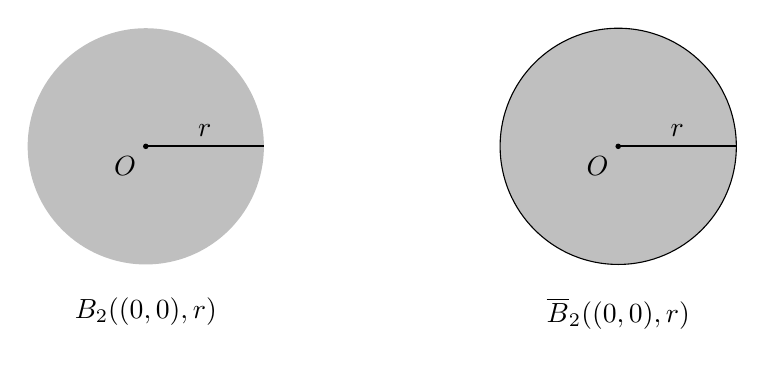
\begin{tikzpicture}

%--- Open ball: B_2((0,0),r) ---
\begin{scope}[shift={(-3,0)}] % shift left
  % Open ball (filled only, no border)
  \fill[gray!50] (0,0) circle (1.5); % radius = r

  % Origin
  \fill (0,0) circle (1pt);
  \node[below left] at (0,0) {$O$};

  % Radius line
  \draw[thick] (0,0) -- (1.5,0) node[midway, above] {$r$};

  % Label below
  \node[below] at (0,-1.8) {$B_2((0,0),r)$};
\end{scope}

%--- Closed ball: \overline{B}_2((0,0),r) ---
\begin{scope}[shift={(3,0)}] % shift right
  % Closed ball (filled + border)
  \filldraw[fill=gray!50, draw=black] (0,0) circle (1.5); % radius = r

  % Origin
  \fill (0,0) circle (1pt);
  \node[below left] at (0,0) {$O$};

  % Radius line
  \draw[thick] (0,0) -- (1.5,0) node[midway, above] {$r$};

  % Label below
  \node[below] at (0,-1.8) {$\overline{B}_2((0,0),r)$};
\end{scope}

\end{tikzpicture}
\end{center}

\item Consideremos bolas abiertas y cerradas con la métrica 'del taxi': 
	\[ B_{1}\left(\left(0,0\right), r\right) = \left\{ \left(x,y\right) \; : \; \left|x\right| + \left|y\right| < r\right\} , \; \overline{B}_{1}\left(\left(0,0\right), r\right) = \left\{ \left(x,y\right) \; : \; \left|x\right| + \left|y\right| \leq r\right\}.\]
	\begin{center}
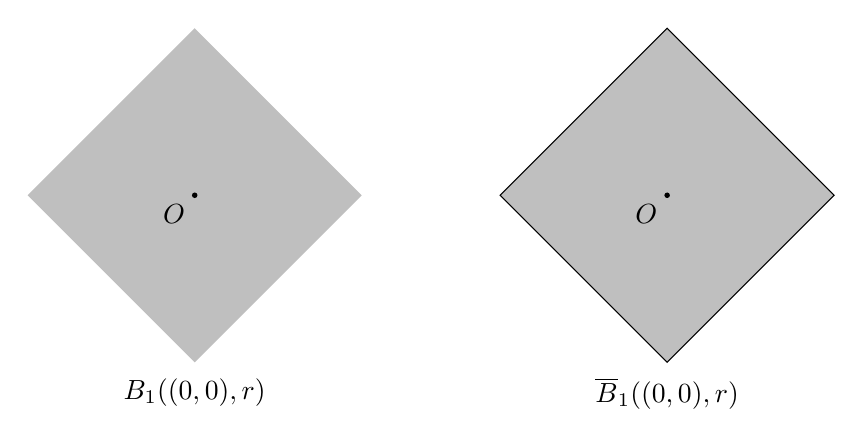
\begin{tikzpicture}
%--- Open L1 ball: B_1((0,0),r) ---
\begin{scope}[shift={(-3,0)}, rotate=45] % left, rotated 45 degrees
  % Filled square, no border
  \fill[gray!50] (-1.5,-1.5) rectangle (1.5,1.5);
  % Origin
  \fill (0,0) circle (1pt);
  \node[below left] at (0,0) {$O$};
\end{scope}
\node[below] at (-3,-2.2) {$B_1((0,0),r)$};
%--- Closed L1 ball: \overline{B}_1((0,0),r) ---
\begin{scope}[shift={(3,0)}, rotate=45] % right, rotated 45 degrees
  % Filled square, with border
  \filldraw[fill=gray!50, draw=black] (-1.5,-1.5) rectangle (1.5,1.5);
  % Origin
  \fill (0,0) circle (1pt);
  \node[below left] at (0,0) {$O$};
\end{scope}
\node[below] at (3,-2.2) {$\overline{B}_1((0,0),r)$};
\end{tikzpicture}	
	\end{center}
	
\item Consideremos bolas abiertas y cerradas con la métrica infinita:
	\[ B_{\infty}\left(\left(0,0\right), r\right) = \left\{ \left(x,y\right) \; : \; \max \left\{ \left|x\right|, \left|y\right|\right\} < r\right\} = \left\{ \left(x,y\right) \; : \; \left|x\right|, \left|y\right| < r\right\} .\]
	\[\overline{B}_{\infty}\left(\left(0,0\right), r\right) = \left\{ \left(x,y\right) \; : \; \max \left\{ \left|x\right|, \left|y\right|\right\} \leq r\right\} = \left\{ \left(x,y\right) \; : \; \left|x\right|, \left|y\right| \leq r\right\}  .\]
\begin{center}
	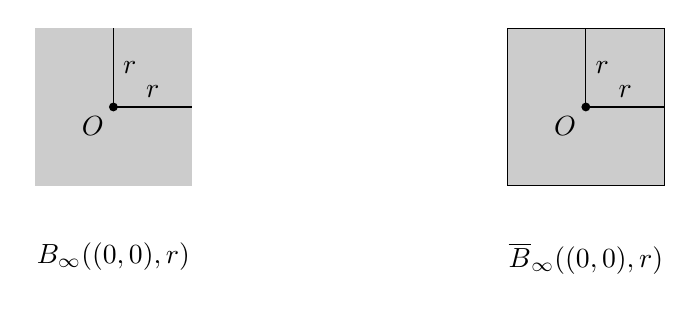
\begin{tikzpicture}[scale=2]

%--- Open L∞ ball: B∞((0,0),r) ---
\begin{scope}[shift={(-1.5,0)}] % shift left, closer
  % Square (filled only, no border)
  \fill[gray!40] (-0.5,-0.5) rectangle (0.5,0.5);

  % Origin
  \fill (0,0) circle (0.8pt);
  \node[below left] at (0,0) {$O$};

  % Radius lines
  \draw (0,0) -- (0,0.5) node[midway,right] {$r$};
  \draw (0,0) -- (0.5,0) node[midway,above] {$r$};

  % Label
  \node[below] at (0,-0.8) {$B_{\infty}((0,0),r)$};
\end{scope}

%--- Closed L∞ ball: \overline{B}∞((0,0),r) ---
\begin{scope}[shift={(1.5,0)}] % shift right, closer
  % Square (filled + border)
  \filldraw[fill=gray!40, draw=black] (-0.5,-0.5) rectangle (0.5,0.5);

  % Origin
  \fill (0,0) circle (0.8pt);
  \node[below left] at (0,0) {$O$};

  % Radius lines
  \draw (0,0) -- (0,0.5) node[midway,right] {$r$};
  \draw (0,0) -- (0.5,0) node[midway,above] {$r$};

  % Label
  \node[below] at (0,-0.8) {$\overline{B}_{\infty}((0,0),r)$};
\end{scope}

\end{tikzpicture}
\end{center}
	
\end{enumerate}
\end{eg}
\begin{observation}
	En $\displaystyle \left(\R, \left| \cdot \right|\right) $ se tiene que $\displaystyle B\left(0,r\right) = \left(-r,r\right) $ y $\displaystyle \overline{B}\left(0,r\right) = \left[-r,r\right]  $. Similarmente, tenemos que $\displaystyle B\left(a,r\right) = \left(a-r, a + r\right) $ y $\displaystyle \overline{B}\left(a,r\right) = \left[a - r, a + r\right]  $.
\end{observation}
\begin{observation}[Relación de las bolas en $\displaystyle \R^n $]
Sabemos que 
\[\|x\|_{\infty} \leq \|x\|_{2} \leq \|x\|_{1} \leq n \|x\|_{\infty} .\]
Por tanto, tenemos que 
\[B_{1}\left(a,r\right) \subset B_{2}\left(a,r\right) \subset B_{\infty}\left(a,r\right) \subset B_{1}\left(a, nr\right) \footnote{También se puede escribir $\displaystyle B_{\infty}\left(a,nr\right) \subset B_{1}\left(a,r\right) \subset B_{2}\left(a,r\right) \subset B_{\infty}\left(a,nr\right) $ .}  .\]
En efecto, si $\displaystyle x \in B_{1} \left(a,r\right) $, tenemos que $\displaystyle \|x - a\|_{1} < r $. Por tanto, es fácil ver que $\displaystyle \|x - a\|_{2} \leq \|x - a\|_{1} < r $, por lo que $\displaystyle x \in B_{2}\left(a,r\right) $. El resto de inclusiones se deducen de forma análoga.
\end{observation}
\begin{definition}
Sean $\displaystyle \left(X,d\right) $ un espacio métrico y $\displaystyle A \subset X $. Se define el \textbf{diámetro} de $\displaystyle A $ como 
\[diam\left(A\right) = \sup \left\{ d\left(x,y\right) \; : \; x,y \in A\right\} \in [0, \infty) .\]
Se dice que $\displaystyle A $ es \textbf{acotado} si $\displaystyle diam\left(A\right) < \infty $.
\end{definition}
\begin{prop}
Dado un espacio métrico $\displaystyle \left(X,d\right) $ con $\displaystyle A \subset X $, tenemos que $\displaystyle A $ está acotado si y solo si $\displaystyle A $ está contenido en alguna bola.
\end{prop}
\begin{proof}
\begin{description}
\item[(i)] Supongamos que $\displaystyle A $ está acotado, entonces $\displaystyle diam\left(A\right) = r < \infty $. Así, tenemos que si $\displaystyle x \in A $, etonces $\displaystyle \forall a \in A $ se tiene que $\displaystyle d\left(a,x\right) \leq r $, por lo que $\displaystyle A \subset \overline{B}\left(a,r\right) $. También podemos ver que lo contiene una bola abierta: $\displaystyle A \subset \overline{B}\left(a, r\right) \subset B\left(a, r+1\right) $.
\item[(ii)] Si $\displaystyle A $ está contenido en una bola, tenemos que existe $\displaystyle x \in X $ y $\displaystyle \frac{r}{2}>0 $ tal que $\displaystyle A \subset B\left(x, \frac{r}{2}\right) $. De esta manera, si $\displaystyle a,b \in A $ se tiene que 
	\[d\left(a,b\right) \leq d\left(a,x\right) + d\left(x,b\right) < \frac{r}{2} + \frac{r}{2} = r .\]
	Así, se tiene que $\displaystyle \forall a,b \in A $, $\displaystyle d\left(a,b\right) < r $, por lo que $\displaystyle diam\left(A\right) \leq r < \infty $, por lo que $\displaystyle A $ está acotado.
\end{description}
\end{proof}

\section{Conceptos topológicos}
\begin{definition}[Conjunto abierto]
Sean $\displaystyle \left(X,d\right) $ un espacio métrico y $\displaystyle A \subset X $. Se dice que $\displaystyle A $ es un \textbf{conjunto abierto} si $\displaystyle \forall a \in A, \exists r> 0 $ tal que $\displaystyle B\left(a,r\right) \subset A $.
\end{definition}
\begin{prop}
Toda bola abierta es un conjunto abierto.
\end{prop}
\begin{proof}
	Tomemos $\displaystyle A = B\left(a,R\right) $ y $\displaystyle x \in B\left(a,R\right) $. Sea $\displaystyle \delta = d\left(x, a\right) < R $ y $\displaystyle r = R - \delta > 0 $ \footnote{No hace falta de escribir $\displaystyle r = \min \left\{ R - \delta, \delta \right\} $ al tratarse de una bola.}. Sea $\displaystyle y \in B\left(x,r\right) $, tenemos que $\displaystyle d\left(x,y\right) < r $. Así, 
\[d\left(y,a\right) \leq d\left(y,x\right) + d\left(x,a\right) < r + \delta = R .\]
Así, $\displaystyle y \in B\left(a,R\right) $, por lo que $\displaystyle B\left(x,r\right) \subset B\left(a,R\right) $.
\end{proof}
\begin{eg}
En $\displaystyle \left(\R^{2}, \| \cdot \|_{2}\right) $.
\begin{enumerate}
	\item Consideremos $\displaystyle A = \left\{ \left(x,y\right) \; : \; 0 < x < 1\right\}  $. Vamos a ver que es abierto. Si $\displaystyle a \in A $, sea $\displaystyle a = \left(x,y\right) $ y consideramos $\displaystyle r = \min \left\{ x, 1 - x\right\}  $. Entonces, tenemos que $\displaystyle B_{2}\left(a,r\right) \subset A $, en efecto, si $\displaystyle \left(x', y'\right) \in B_{2}\left(a,r\right) $:
\[\sqrt{\left(x-x'\right)^{2} + \left(y-y'\right)^{2}} < r \Rightarrow \left|x - x'\right| < r \Rightarrow 0 < x' < 1.\]
Así, tenemos que $\displaystyle \left(x',y'\right)\in A $.
\item Consideremos $\displaystyle A = \left\{ \left(x,y\right) \; : \; 0 < x \leq 1\right\}  $. Vamos a ver que no es abierto. En efecto, si tomamos $\displaystyle a = \left(1,0\right) $ y $\displaystyle r > 0 $,
	tenemos que $\displaystyle \left(1 + \frac{r}{2}, 0\right) \in B_{2}\left(a,r\right) $ pero $\displaystyle \left(1 + \frac{r}{2}, 0\right) \not\in A $. 
\end{enumerate}
\end{eg}
\begin{prop}
En $\displaystyle \R^{n} $ los conjuntos abiertos coinciden para $\displaystyle \| \cdot \|_{1} $, $\displaystyle \| \cdot \|_{2} $ y $\displaystyle \| \cdot \|_{\infty} $.
\end{prop}
\begin{proof}
Como se vio en una observación anterior, sabemos que 
\[B_{1}\left(a,r\right) \subset B_{2}\left(a,r\right) \subset B_{\infty}\left(a,r\right) \subset B_{1}\left(a,nr\right) .\]
\begin{itemize}
\item Sea $\displaystyle A \subset \R^{n} $. Si $\displaystyle A $ es abierto con la norma $\displaystyle \| \cdot \|_{2} $, tenemos que $\displaystyle \forall a \in A, \exists r > 0 $ tal que $\displaystyle B_{2}\left(a,r\right) \subset A $. Por la observación, como $\displaystyle B_{1}\left(a,r\right) \subset B_{2}\left(a,r\right) \subset A $, tenemos que también es abierto para la norma $\displaystyle \| \cdot \|_{1} $.
\item Sea $\displaystyle A \subset \R^{n} $. Si $\displaystyle A $ es abierto con la norma $\displaystyle \| \cdot \|_{\infty} $, entonces $\displaystyle \forall a \in A, \exists r > 0 $ tal que $\displaystyle B_{\infty}\left(a,r\right) \subset A $. Por la observación anterior, tenemos que $\displaystyle B_{2}\left(a,r\right) \subset B_{\infty}\left(a,r\right) \subset A $, por lo que $\displaystyle A $ es abierto respecto a la norma $\displaystyle \| \cdot \|_{2} $.
\item Sea $\displaystyle A \subset \R^{n} $. Si $\displaystyle A $ es abierto respecto de $\displaystyle \| \cdot \|_{1} $, tenemos que $\displaystyle \forall a \in A, \exists r > 0 $ tal que $\displaystyle B_{1}\left(a,r\right) \subset A $. Sea $\displaystyle r' = \frac{r}{n} > 0 $, 
	\[B_{\infty}\left(a,r'\right)\subset B_{1}\left(a, nr'\right) = B_{1}\left(a,r\right) \subset A.\]
	Por tanto, $\displaystyle A $ es abierto respecto de la norma $\displaystyle \| \cdot \| _{\infty} $.
\end{itemize}
\end{proof}
\begin{theorem}[Propiedades de los abiertos]
Sea $\displaystyle \left(X,d\right) $ un espacio métrico. 
\begin{enumerate}
\item $\displaystyle X $ y $\displaystyle \emptyset $ son abiertos.
\item La unión arbitraria de abiertos es abierto.
\item La intersección finita de abiertos es abierto.
\end{enumerate}
\end{theorem}
\begin{proof}
\begin{enumerate}
\item Es trivial que $\displaystyle \emptyset $ es abierto. Por otro lado, si $\displaystyle a \in X $, tenemos que $\displaystyle \forall r > 0 $, $\displaystyle B\left(x,r\right) \subset X $. Así, $\displaystyle X $ está abierto.
\item Supongamos que $\displaystyle \left\{ A_{i}\right\}_{i \in I} $ es una familia de conjuntos abiertos y sea $\displaystyle A = \bigcup_{i \in I}A_{i} $. Si $\displaystyle a \in A $, tenemos que $\displaystyle a \in A_{i} $ para algún $\displaystyle i \in I $. Así, existe $\displaystyle r>0 $ tal que $\displaystyle B \left(a,r\right) \subset A_{i} \subset \bigcup_{i \in I}A_{i}$. Por tanto, $\displaystyle B\left(a,r\right) \subset A $ y $\displaystyle A $ es abierto.
\item Sean $\displaystyle A_{1}, \ldots, A_{m} $ conjuntos abiertos y sea $\displaystyle A = A_{1} \cap \cdots \cap A_{m} $. Si $\displaystyle a \in A $, tenemos que $\displaystyle a \in A_{i} $ para $\displaystyle 1 \leq i \leq m $.
	Así, existe $\displaystyle r_{i} > 0 $ tal que $\displaystyle B\left(a, r_{i}\right) \subset A_{i} $. Si tomamos $\displaystyle r = \min \left\{ r_{i} \; : \; 1 \leq i \leq m\right\}  $, tenemos que $\displaystyle B\left(a, r\right) \subset B\left(a, r_{i}\right) $, $\displaystyle \forall i = 1, \ldots, m $. Por tanto, $\displaystyle B\left(a,r\right) \subset A $ y $\displaystyle A $ es abierto.
\end{enumerate}
\end{proof}
\begin{observation}
La intersección infinita de conjuntos abiertos puede no ser abierto. Por ejemplo, consideremos en $\displaystyle \left(\R^{2}, \| \cdot \|_{2}\right) $ consideramos $\displaystyle A_{m} = B_{2}\left(\left(0,0\right), \frac{1}{m}\right) $, que es abierto $\displaystyle \forall m \in M $.
Sin embargo, $\displaystyle A = \bigcap_{m = 1}^{\infty}A_{m} = \left\{ \left(0,0\right)\right\}  $, que no es abierto.
\end{observation}
\begin{definition}[Conjunto cerrado]
Sea $\displaystyle \left(X,d\right) $ un espacio métrico. Se dice que un conjunto $\displaystyle C \subset X $ es \textbf{cerrado} si $\displaystyle X/C $ es abierto.
\end{definition}
\begin{prop}
Toda bola cerrada es un conjunto cerrado.
\end{prop}
\begin{proof}
En efecto, sea $\displaystyle C = \overline{B}\left(p, R\right) = \left\{ x \in X \; : \; d\left(x,p\right) \leq R\right\}  $ y sea $\displaystyle A = X/C = \left\{ x \in X \; : \; d\left(x, p\right) > R\right\}  $. Si $\displaystyle a \in A $, tenemos que $\displaystyle d\left(a,p\right) = \delta > R $. Así, tomando $\displaystyle r = \delta - R > 0 $, si $\displaystyle x\in B\left(a,r\right)  $, tenemos que 
	 \[
	 \begin{split}
	 d\left(x,p\right) \geq d\left(p,a\right)- d\left(x,a\right) > \delta - r = R.
	 \end{split}
	 \]
	 Así, tenemos que $\displaystyle x \in A $, por lo que $\displaystyle B\left(a,r\right) \subset A $ y $\displaystyle X/C $ es abierto, por lo que $\displaystyle C $ es cerrado.
\end{proof}
\begin{observation}
Es fácil ver que en $\displaystyle \left(\R, | \cdot |\right) $:
\begin{itemize}
\item $\displaystyle \left(a,b\right) $ es abierto.
\item $\displaystyle \left[a,b\right]  $ es cerrado.
\item $\displaystyle (a,b]  $ y $\displaystyle [a,b) $ no son ni abiertos ni cerrados.
\end{itemize}
\end{observation}
\begin{theorem}[Propiedades de los cerrados]
Sea $\displaystyle \left(X, \emptyset\right) $ un espacio métrico.
\begin{enumerate}
\item Los conjuntos $\displaystyle X $ y $\displaystyle \emptyset $ son cerrados.
\item La intersección arbitraria de cerrados es cerrado.
\item La unión finita de cerrados es cerrado.
\end{enumerate}
\end{theorem}
\begin{proof}
\begin{enumerate}
\item Dado que $\displaystyle \emptyset = X/X $ y $\displaystyle X = X/\emptyset $, del teorema anterior se sigue que son cerrados.
\item Sean $\displaystyle \left\{ C_{i}\right\} _{i \in I} $ cerrados. Entonces, $\displaystyle \forall i \in I $ tenemos que $\displaystyle X/C_{i} $ es abierto, así,
	\[X/\bigcap_{i \in I}C_{i} = \bigcup_{i \in I}\left(X/C_{i}\right) ,\]
	que es abierto, por lo que $\displaystyle \bigcap_{i \in I}C_{i} $ es cerrado.
\item Sean $\displaystyle C_{1}, \ldots, C_{m} $ cerrados. Entonces, $\displaystyle \forall i = 1, \ldots, m $, tenemos que $\displaystyle X/C_{i} $ es abierto. Así,
	\[X/\bigcup_{i = 1}^{m}C_{i} = \bigcap_{i = 1}^{m}\left(X/C_{i}\right) ,\]
	es abierto, por lo que $\displaystyle \bigcup_{i = 1}^{m}C_{i} $ es cerrado.
\end{enumerate}
\end{proof}
\begin{definition}[Punto interior]
Sea $\displaystyle \left(X,d\right) $ un espacio métrico y $\displaystyle A \subset X $. Se dice que $\displaystyle a \in A $ es un \textbf{punto interior} de $\displaystyle A $ si existe $\displaystyle r > 0 $ tal que $\displaystyle B\left(a,r\right) \subset A $. Denotamos $\displaystyle \Int\left(A\right) $ al conjunto de puntos interiores de $\displaystyle A $.
\end{definition}
\begin{observation}
Es trivial ver que $\displaystyle \Int\left(A\right) \subset A $. 
\end{observation}
\begin{prop}
Sea $\displaystyle \left(X,d\right) $ un espacio métrico y $\displaystyle A \subset X $.
\begin{enumerate}
\item El conjunto $\displaystyle \Int\left(A\right) $ es el mayor abierto contenido en A.
\item $\displaystyle A $ es abierto si y solo si $\displaystyle A = \Int\left(A\right) $.
\end{enumerate}
\end{prop}

\begin{proof}
\begin{enumerate}
\item Sea $\displaystyle U = \Int\left(A\right) $. Vamos a ver que es abierto. Dado $\displaystyle x \in U $, tenemos que existe $\displaystyle r > 0 $ tal que $\displaystyle B\left(x,r\right) \subset A $. Si $\displaystyle y \in B\left(x,r\right) $, por tratarse de una bola abierta existe $\displaystyle r' > 0 $ tal que $\displaystyle B\left(y,r'\right)\subset B\left(x,r\right) \subset A $, por lo que $\displaystyle y \in \Int\left(A\right) = U $. Por tanto, $\displaystyle B\left(x,r\right) \subset U $ y $\displaystyle U $  es abierto. \\ 
	Ahora tenemos que ver que es el mayor abierto. Supongamos que $\displaystyle V $ es abierto y $\displaystyle V \subset A $. Sea $\displaystyle x \in V $, tenemos que existe $\displaystyle r > 0 $ tal que $\displaystyle B\left(x,r\right) \subset V \subset A$. Por tanto, $\displaystyle x \in \Int\left(A\right) = U$ y $\displaystyle V \subset U $.
\item Si $\displaystyle A = Int\left(A\right) $ está claro que $\displaystyle A $ es abierto. Recíprocamente, si $\displaystyle A $ es abierto, tenemos que como $\displaystyle A $ es el mayor abierto contenido en $\displaystyle A $, $\displaystyle A = Int\left(A\right) $.
\end{enumerate}
\end{proof}
\begin{eg}
	En $\displaystyle \left(\R, \left| \cdot \right|\right) $, sea $\displaystyle A = (0,2] $. Tenemos que $\displaystyle \Int\left(A\right) = \left(0,2\right) $. En efecto, 
	\begin{description}
		\item[(i)] Si $\displaystyle x \in \left(0,2\right) $, entonces existe $\displaystyle r > 0 $ tal que $\displaystyle \left(x -r, x+r\right) \subset \left(0,2\right) \subset (0,2] $, por lo que $\displaystyle x \in \Int\left(A\right) $.
	\item[(ii)] Recíprocamente, tenemos que $\displaystyle 2 \not\in \Int\left(A\right) $, puesto que $\displaystyle \forall r > 0 $ tenemos que $\displaystyle \left(2-r, 2 + r\right)$ no es subconjunto de $ (0,2] $.
	\end{description}
\end{eg}
\begin{definition}[Punto adherente]
Sean $\displaystyle \left(X,d\right) $ un espacio métrico y $\displaystyle A \subset X $. Se dice que $\displaystyle x \in X $ es \textbf{punto adherente} a $\displaystyle A $ (o también \textbf{punto clausura}) si $\displaystyle \forall r > 0 $, $\displaystyle A \cap B\left(x,r\right) \neq \emptyset $. Denotamos $\displaystyle \overline{A} $ o $\displaystyle Adh\left(A\right) $ al conjunto de puntos adherentes de $\displaystyle A $.
\end{definition}
\begin{observation}
Se ve trivialmente que $\displaystyle A \subset \overline{A} $.
\end{observation}
\begin{eg}
	En $\displaystyle \left(\R, \left| \cdot \right|\right) $ sea $\displaystyle A = (0,2] $. Tenemos que $\displaystyle \overline{A} = \left[0,2\right]  $. En efecto:
	\begin{description}
	\item[(i)] Tenemos que $\displaystyle 0 \in \overline{A} $, puesto que $\displaystyle \forall r > 0 $ tenemos que $\displaystyle \left(-r,r\right) \cap A \neq \emptyset $. Así, tenemos que $\displaystyle \left[0,2\right] \subset \overline{A} $.
	\item[(ii)] Recíprocamente, si $\displaystyle x > 2 $, tenemos que existe $\displaystyle r > 0 $ suficientemente pequeño tal que $\displaystyle x - r > 2 $, por tanto $\displaystyle x \not\in \overline{A} $. Similarmente, podemos demostrar que $\displaystyle 0 \not\in \overline{A} $.
	\end{description}
\end{eg}
\begin{lema}
Sean $\displaystyle \left(X,d\right) $ un espacio métrico y $\displaystyle A \subset X $. Entcones, $\displaystyle \overline{A} = X/\Int\left(X/A\right) $.
\end{lema}
\begin{proof}
\begin{description}
\item[(i)] Sea $\displaystyle x \in \overline{A} $. Tenemos que $\displaystyle \forall r > 0 $, $\displaystyle B\left(x,r\right) \cap A \neq \emptyset $, por lo que $\displaystyle B\left(x,r\right) \not \subset X/A $, por lo que $\displaystyle x \not\in \Int\left(X/A\right) $, por lo que $\displaystyle x \in X/\Int\left(X/A\right) $.
\item[(ii)] Sea $\displaystyle x \in X/\Int\left(X/A\right) $, entonces $\displaystyle x \not\in \Int\left(X/A\right) $, es decir, $\displaystyle \forall r > 0 $ tenemos que $\displaystyle B\left(x,r\right) \not \subset X/A $. Así, debe ser que $\displaystyle B\left(x,r\right) \cap A \neq \emptyset $, por lo que $\displaystyle x \in \overline{A} $.
\end{description}
\end{proof}
\begin{prop}
\begin{enumerate}
\item $\displaystyle \overline{A} $ es el menor cerrado que contiene a $\displaystyle A $.
\item Un conjunto $\displaystyle A \subset X $ es cerrado si y solo si $\displaystyle A = \overline{A} $.
\end{enumerate}
\end{prop}
\begin{proof}
\begin{enumerate}
\item Tenemos que $\displaystyle \overline{A} = X/\Int\left(X/A\right) $, por lo que su complementario es abierto y él es cerrado. Ahora vamos a ver que es el menor cerrado que contiene a $\displaystyle A $. Sea $\displaystyle C \subset X $ cerrado con $\displaystyle A \subset C $. Tenemos que $\displaystyle X/C \subset X/A $, por lo que $\displaystyle X/C \subset \Int\left(X/A\right) $ y tenemos que $\displaystyle C \supset X/\Int\left(X/A\right) = \overline{A} $.
\item Si $\displaystyle A = \overline{A} $, $\displaystyle A  $ es cerrado.
Por otro lado, si $\displaystyle A $ es cerrado, entonces su complementario, $\displaystyle X/A $ es abierto, por lo que $\displaystyle X/A = \Int\left(X/A\right) $, por lo que $\displaystyle \overline{A} = X/\Int\left(X/A\right) = X/\left(X/A\right) = A $.
\end{enumerate}
\end{proof}
\begin{definition}[Punto frontera]
Sean $\displaystyle \left(X,d\right) $ un espacio métrico y $\displaystyle A \subset X $. Se dice que $\displaystyle x \in X $ es un \textbf{punto frontera} de $\displaystyle A $ si $\displaystyle \forall r > 0 $, $\displaystyle B\left(x,r\right) \cap A \neq \emptyset $ y $\displaystyle B\left(x,r\right) \cap \left(X/A\right) \neq \emptyset $. Denotamos $\displaystyle Fr\left(A\right) $ o $\displaystyle \partial A$ el conjunto de puntos frontera de $\displaystyle A $.
\end{definition}
\begin{observation}
Tenemos que $\displaystyle Fr\left(A\right) = \overline{A} \cap \overline{X/A} $ y en particular $\displaystyle Fr\left(A\right) $ es cerrado.
\end{observation}
\begin{eg}
	En $\displaystyle \left(\R^{2}, \| \cdot \|_{2}\right) $ sea $\displaystyle A = \left\{ \left(x,y\right) \; : \; 0 < x \leq 1\right\}  $.Tenemos que  
	\[ Fr\left(A\right) = \left\{ \left(0,y\right)\; : \; y \in \R\right\} \cup \left\{ \left(1,y\right) \; : \; y \in \R\right\} .\]
	En efecto:
	\begin{description}
	\item[(i)] Sea $\displaystyle P = \left(0,y\right) $. Tenemos que $\displaystyle \forall r > 0 $, $\displaystyle B\left(P,r\right) \cap A \neq \emptyset $ y $\displaystyle B\left(P,r\right)\cap \left(X/A\right) \neq \emptyset $. Así, $\displaystyle P \in Fr\left(A\right) $. De forma análoga, se puede demostrar que $\displaystyle P = \left(1,y\right) \in Fr\left(A\right) $.
	\item[(ii)] El recíproco lo demostramos típicamente por contrapositiva. Sea $\displaystyle P = \left(x,y\right) \in \R^{2} $ con $\displaystyle x \neq 0 $ y $\displaystyle x \neq 1 $. Hay tres posibilidades a considerar: $\displaystyle x \in \left(-\infty, 0\right) $, $\displaystyle x \in \left(0,1\right) $ o $\displaystyle x \in \left(1,\infty\right) $. Si $\displaystyle x \in \left(-\infty, 0\right) $, $\displaystyle \exists r > 0 $ tal que $\displaystyle B\left(P,r\right) \cap A = \emptyset $. El resto de los casos se demuestran de forma análoga.
	\end{description}
\end{eg}
\begin{definition}[Punto de acumulación]
	Sean $\displaystyle \left(X,d\right) $ un espacio métrico y $\displaystyle A \subset X $. Se dice que $\displaystyle x \in X $ es un \textbf{punto de acumulación} de $\displaystyle A $ si $\displaystyle \forall r> 0 $ se tiene que $\displaystyle A \cap \left(B\left(x,r\right)/ \left\{ x\right\} \right)\neq \emptyset $. Denotamos $\displaystyle A' $ el conjunto de los puntos de acumulación de $\displaystyle A $.
\end{definition}
\begin{observation}
	Tenemos que $\displaystyle A' \subset \overline{A} $. En efecto, si $\displaystyle x \in A' $, tenemos que $\displaystyle \forall r > 0 $ se cumple que $\displaystyle A \cap \left(B\left(x,r\right) / \left\{ x\right\} \right) \neq \emptyset $, es decir, $\displaystyle A \cap B\left(x,r\right) \neq \emptyset $, por lo que $\displaystyle x \in \overline{A} $.
\end{observation}
\begin{eg}
Consideremos $\displaystyle A = \N \times \N \subset \left(\R^{2}, d _{2}\right)$. Tenemos que 
\begin{itemize}
\item $\displaystyle \Int\left(A\right) = \emptyset $. En efecto, tenemos que $\displaystyle \forall r > 0 $, si $\displaystyle n_{0} = \left(n,n\right) \in \N^{2} $, existe $\displaystyle x \in \R/\Q $ tal que $\displaystyle n < x < n + r $, por lo que $\displaystyle \left(x,x\right) \in B\left(n,r\right) $ pero $\displaystyle \left(x,x\right)\not\in \N^{2} $.
\item $\displaystyle \overline{A} = A $. En efecto, si $\displaystyle x \not\in A$, tenemos que podemos encontrar $\displaystyle r > 0 $ suficientemente pequeño tal que $\displaystyle B\left(x,r\right) \cap A = \emptyset $.
\item $\displaystyle \partial A = A $. Dado que $\displaystyle A = \overline{A} $ y $\displaystyle \partial A= \overline{A} \cap \overline{X/A} $, tenemos que $\displaystyle A \subset \partial A $. Por otro lado, si $\displaystyle x \not\in A $, tenemos que existe un $\displaystyle r>0 $ suficientemente pequeño tal que $\displaystyle B\left(x,r\right) \cap A = \emptyset $, como hemos visto anteriormente, por lo que $\displaystyle x \not\in \partial A $. 
\item $\displaystyle A' = \emptyset $. Si cogemos $\displaystyle r < 1 $ y $\displaystyle n \in \N^{2} $, está claro que $\displaystyle \left(B\left(n,r\right)/ \left\{ n\right\} \right) \cap A = \emptyset $, por lo que $\displaystyle n $ no puede ser un punto de acumulación. Si $\displaystyle x \not\in A $, hacemos un argumento similar al del apartado anterior.
\end{itemize}
\end{eg}
\begin{definition}[Punto aislado]
	Sean $\displaystyle \left(X,d\right) $ un espacio métrico y $\displaystyle A \subset X $. Se dice que $\displaystyle x \in A $ es un \textbf{punto aislado} de $\displaystyle A $ si existe $\displaystyle r > 0 $ tal que $\displaystyle B\left(x,r\right) \cap A = \left\{ x\right\}  $. Denotaremos $\displaystyle Ais\left(A\right) $ al conjunto de los puntos aislados de $\displaystyle A $.
\end{definition}
\begin{prop}
Sean $\displaystyle \left(X, d\right) $ un espacio métrico y $\displaystyle A \subset X $. Entonces, se cumple que $\displaystyle \overline{A} = A' \cup Ais\left(A\right) $.
\end{prop}
\begin{proof}
\begin{description}
	\item[(i)] Sea $\displaystyle x \in \overline{A} $. Supongamos que $\displaystyle x \not\in A' $, entonces existe $\displaystyle r > 0 $ tal que $\displaystyle A \cap \left(B\left(x,r\right)/ \left\{ x\right\} \right) = \emptyset $. Sin embargo, sabemos que $\displaystyle A \cap B\left(x,r\right) \neq \emptyset $ al ser $\displaystyle x \in \overline{A} $, por tanto debe ser que $\displaystyle A \cap B\left(x,r\right) = \left\{ x\right\}  $, es decir, $\displaystyle x \in Ais\left(A\right) $.
\item[(ii)] Está claro que $\displaystyle Ais\left(A\right) \subset A \subset \overline{A} $ y $\displaystyle A' \subset \overline{A} $, por lo que $\displaystyle A' \cup Ais\left(A\right) \subset \overline{A} $.
\end{description}
\end{proof}
\begin{colorary}
Sean $\displaystyle \left(X,d\right) $ un espacio métrico y $\displaystyle A \subset X $. Entonces, $\displaystyle A $ es cerrado si y solo si $\displaystyle A $ contiene todos sus puntos de acumulación.
\end{colorary}
\begin{proof}
\begin{description}
\item[(i)] Tenemos que $\displaystyle A = \overline{A} = A' \cup Ais\left(A\right)  $, por lo que $\displaystyle A' \subset A $.
\item[(ii)] Tenemos que $\displaystyle Ais\left(A\right) \subset A $ y $\displaystyle A' \subset A $, por lo que $\displaystyle \overline{A} = Ais\left(A\right) \cup A' \subset A $, así, $\displaystyle \overline{A} = A $.
\end{description}
\end{proof}
\begin{definition}
	Sean $\displaystyle \left(x,d\right) $ un espacio métrico, $\displaystyle A \subset X $ y $\displaystyle x \in X $. Se define la \textbf{distancia} de $\displaystyle x $ a $\displaystyle A $ como:
\[d\left(x,A\right) = \inf \left\{ d\left(x,a\right) \; : \; a \in A\right\}  .\]
\end{definition}
\begin{prop}
	Sean $\displaystyle \left(X,d\right) $ un espacio métrico y $\displaystyle A \subset X $. Entonces, 
	\[ \overline{A} = \left\{ x \in X \; : \; d\left(x,A\right) = 0\right\}.\]
\end{prop}
\begin{proof}
\begin{description}
\item[(i)] Sea $\displaystyle x \in \overline{A} $, entonces existe $\displaystyle r > 0 $ tal que $\displaystyle A \cap B\left(x,r\right) \neq \emptyset$. Por tanto, existe $\displaystyle a_{r} \in A \cap B\left(x,r\right) $, por tanto $\displaystyle d\left(x,a_{r}\right) < r $. Así, tenemos que 
	\[ d\left(x,A\right) \leq d\left(x,a_{r}\right) < r, \; \forall r > 0 .\]
	Por tanto, $\displaystyle d\left(x,A\right) = 0 $.
\item[(ii)] Tenemos que $\displaystyle \forall r > 0 $, $\displaystyle d\left(x,A\right) < r $, por lo que existe $\displaystyle a_{r} \in A $ tal que $\displaystyle d\left(x,a_{r}\right)< r $. Por tanto, $\displaystyle a_{r} \in A \cap B\left(x,r\right) \neq \emptyset $ y podemos concluir que $\displaystyle x \in \overline{A} $.
\end{description}
\end{proof}
\section{Conjuntos abiertos y cerrados relativos}
\begin{observation}
Sean $\displaystyle \left(X,d\right) $ un espacio métrico e $\displaystyle Y \subset X $. Sabemos que $\displaystyle \left(Y, d _{Y}\right) $ es un subespacio métrico de $\displaystyle \left(X,d\right) $ donde $\displaystyle d _{Y}\left(y_{1}, y_{2}\right) = d\left(y_{1}, y_{2}\right) $. 
Dado $\displaystyle y_{0} \in Y $ y $\displaystyle r > 0 $, la bola $\displaystyle B_{Y}\left(y_{0}, r\right) = \left\{ y \in Y \; : \; d\left(y, y_{0}\right)<r\right\} = B\left(y_{0}, r\right) \cap Y $. Es decir, la forma de las bolas cambia.
\end{observation}
\begin{observation}
En un espacio métrico $\displaystyle \left(X,d\right) $, todo conjunto abierto es unión de bolas abiertas. En efecto, si $\displaystyle A $ es abierto, entonces $\displaystyle \forall a \in A $, existe $\displaystyle r_{a} > 0 $ tal que $\displaystyle B\left(a,r_{a}\right) \subset A $, por lo que $\displaystyle A = \bigcup_{ a \in A}B\left(a,r_{a}\right) $ \footnote{Esta observación se puede reformular diciendo que un subconjunto $\displaystyle A \subset X $ es abierto si y solo si es unión de bolas abiertas.}.
\end{observation}
\begin{prop}
Sean $\displaystyle \left(X,d\right) $ un espacio métrico e $\displaystyle Y \subset X $. 
\begin{description}
\item[(a)] $\displaystyle A \subset Y $ es $\displaystyle d _{Y} $-abierto si y solo si existe $\displaystyle U \subset X $ abierto tal que $\displaystyle A = U \cap Y $.
\item[(b)] $\displaystyle C \subset Y $ es $\displaystyle d _{Y} $-cerrado si y solo si existe $\displaystyle H \subset X $ cerrado tal que $\displaystyle C = H \cap Y $.
\end{description}
Estos conjuntos se llaman \textbf{abiertos y cerrados relativos} de $\displaystyle Y $, respectivamente.
\end{prop}
\begin{proof}
\begin{description}
\item[(a)] Sea $\displaystyle Y \subset X $.
	\begin{description}
	\item[(i)] Tenemos que $\displaystyle \forall y \in A $, existe $\displaystyle r_{y}>0 $ tal que $\displaystyle B_{Y}\left(y,r_{y}\right) \subset A $. Definimos $\displaystyle U = \bigcup_{y \in A}B\left(y,r_{y}\right) $, que es abierto en $\displaystyle \left(X,d\right) $ por ser unión de bolas abiertas.
Veamos que $\displaystyle A = U \cap Y $. Tenemos que si $\displaystyle y \in A $, entonces $\displaystyle y \in B\left(y, r_{y}\right) \subset A \subset U $ (puesto que $\displaystyle B_{Y}\left(y, r_{y}\right) \subset B\left(y, r_{y}\right) $).
Recíprocamente, sea $\displaystyle z \in Y \cap U $, entonces existe $\displaystyle y \in Y $ tal que $\displaystyle z \in B\left(y,r_{y}\right) \cap Y = B_{Y}\left(y,r_{y}\right) \subset A$. Por tanto, $\displaystyle Y \cap U \subset A $.
	\item[(ii)] Dado $\displaystyle y_{0} \in A = U \cap Y $, como $\displaystyle U $ es abierto \footnote{Cuando escribimos abierto y $\displaystyle B\left(x,r\right) $ queremos decir que es $\displaystyle d $-abierto y es la bola en $\displaystyle X $, respectivamente.} , existe $\displaystyle r > 0 $ tal que $\displaystyle B\left(y_{0}, r\right)\subset U $. Por tanto, tenemos que $\displaystyle B_{Y}\left(y_{0}, r\right) = B\left(y_{0}, r\right)\cap Y \subset U \cap Y = A $. Así, hemos visto que $\displaystyle A $ es $\displaystyle d _{Y} $-abierto.
	\end{description}
\item[(b)] Sea $\displaystyle Y \subset X $.
	\begin{description}
	\item[(i)] Sea $\displaystyle C \subset Y $ $\displaystyle d _{Y} $-cerrado, entonces tenemos que $\displaystyle Y/C $ es $\displaystyle d _{Y} $-abierto. Así, existe $\displaystyle U \subset X $ abierto tal que $\displaystyle Y/C = U \cap Y $. Sea $\displaystyle H = X/U $, que es cerrado. Veamos que $\displaystyle C = H \cap Y $:
\[C = Y / \left(Y / C\right) = Y / \left(U \cap Y\right) = Y / U = Y \cap \left(X/U\right) = Y \cap H .\]
\item[(ii)] Si $\displaystyle C = H\cap Y $ con $\displaystyle H $ cerrado en $\displaystyle X $, entonces $\displaystyle X/H $ es abierto. Tenemos que
	\[Y/C = Y / \left(H \cap Y\right) = Y \cap \left(X/H\right) .\]
	Dado que $\displaystyle X/H $ es abierto, por \textbf{(a)} tenemos que $\displaystyle Y/C $ es $\displaystyle d _{Y} $-abierto, por lo que $\displaystyle C $ es $\displaystyle d _{Y} $-cerrado.
	\end{description}
\end{description}
\end{proof}
\section{Sucesiones en espacios métricos}
\begin{definition}[Sucesión y convergencia]
	Sea $\displaystyle \left(X,d\right) $ un espacio métrico. Una \textbf{sucesión} es una aplicación $\displaystyle S : \N \to X $. Si $\displaystyle S\left(n\right) = x_{n} \in X $, denotamos la sucesión por $\displaystyle \left\{ x_{n}\right\} _{n\in\N} $. Se dice que $\displaystyle \left\{ x_{n}\right\} _{n\in\N} $ \textbf{converge} a $\displaystyle x_{0} \in X $ cuando $\displaystyle  d\left(x_{n}, x_{0}\right) _{n\in\N} \to 0 $ 
\end{definition}
\begin{observation}
	Recordamos que $\displaystyle x_{n} \to x_{0} $ si y solo si (ambas definiciones son equivalentes):
\begin{itemize}
\item  $\displaystyle \forall \epsilon > 0 $ existe $\displaystyle n_{0} \in \N $ tal que $\displaystyle \forall n \geq n_{0} $ se tiene que $\displaystyle d\left(x_{n}, x_{0}\right) < \epsilon  $.
\item $\displaystyle \forall \epsilon > 0 $ existe $\displaystyle n_{0} \in \N $ tal que $\displaystyle \forall n \geq n_{0} $ se tiene que $\displaystyle x_{n} \in B\left(x_{0}, \epsilon \right) $.
\end{itemize}
\end{observation}
\begin{prop}
	Sea $\displaystyle \left(X,d\right) $ un espacio métrico. Si la sucesión $\displaystyle \left\{ x_{n}\right\} _{n\in\N} $ converge, el límite es único.
\end{prop}
\begin{proof}
Supongamos que $\displaystyle l_{1}, l_{2} \in X $ son límites de la sucesión, entonces tenemos que si $\displaystyle \epsilon > 0 $, existe $\displaystyle n_{0} \in \N $ tal que $\displaystyle \forall n \geq n_{0} $ se cumple que
\[ d\left(l_{1}, l_{2}\right) \leq d\left(l_{1}, x_{n}\right) + d\left(x_{n}, l_{2}\right) < \frac{\epsilon }{2} + \frac{\epsilon }{2} = \epsilon .\]
Como esto es cierto para todo $\displaystyle \epsilon > 0 $, debe ser que $\displaystyle d\left(l_{1}, l_{2}\right) = 0 $, por lo que $\displaystyle l_{1} = l_{2} $.
\end{proof}
\begin{prop}
	Sea $\displaystyle \left(X,d\right) $ un espacio métrico y $\displaystyle A \subset X $. Entonces, $\displaystyle x \in \overline{A} $ si y solo si existe una sucesión $\displaystyle \left\{ x_{n}\right\} _{n\in\N} \subset A $ tal que $\displaystyle x_{n}\to x $.
\end{prop}
\begin{proof}
\begin{description}
	\item[(i)] Tenemos que si $\displaystyle x \in \overline{A} $, entonces para todo $\displaystyle \epsilon > 0 $ se tiene que $\displaystyle B\left(x,\epsilon \right) \cap A \neq \emptyset $, es decir. Así, podemos coger una sucesión tal que para $\displaystyle \epsilon = \frac{1}{n} $ se tiene que $\displaystyle x_{n} \in B\left(x,\frac{1}{n}\right) \cap A $. Vamos a ver que la sucesión $\displaystyle \left\{ x_{n}\right\} _{n\in\N} $ converge a $\displaystyle x $. 
		\[0 \leq d\left(x_{n}, x\right) < \frac{1}{n} \Rightarrow d\left(x_{n}, x\right) \to 0 \iff x_{n} \to x .\]
	\item[(ii)] Si existe $\displaystyle \left\{ x_{n}\right\} _{n\in\N} \subset A $ tal que $\displaystyle x_{n} \to x $, tenemos que si $\displaystyle r > 0 $, existe $\displaystyle n_{0} \in \N $ tal que $\displaystyle \forall n \geq n_{0} $, $\displaystyle x_{n} \in B\left(x, r\right) $, es decir, $\displaystyle B\left(x,r\right) \cap A \neq \emptyset $, por lo que $\displaystyle x \in \overline{A} $.
\end{description}
\end{proof}
\begin{prop}
	Sea $\displaystyle \left(X,d\right) $ un espacio métrico y $\displaystyle A \subset X $. Entonces $\displaystyle x \in A' $ si y solo si existe una sucesión $\displaystyle \left\{ x_{n}\right\} _{n\in\N} $ de términos distintos con $\displaystyle x_{n} \to x $.
\end{prop}
\begin{proof}
\begin{description}
	\item[(i)] Si $\displaystyle x \in A' $, tenemos que $\displaystyle \forall r> 0 $, $\displaystyle A \cap \left(B\left(x,r\right)/ \left\{ x\right\} \right) \neq \emptyset $. 
		\begin{itemize}
			\item Para $\displaystyle n = 1 $, tomamos $\displaystyle x_{1} $ tal que $\displaystyle x_{1} \in A \cap \left(B\left(x,1\right) / \left\{ x\right\} \right) $.
			\item Para $\displaystyle n = 2 $, tomamos $\displaystyle \epsilon = \min \left\{ \frac{1}{2}, d\left(x_{1}, x\right)\right\}  $, y tomamos $\displaystyle x_{2} $ tal que $\displaystyle x_{2} \in A \cap \left(B\left(x,\epsilon \right) / \left\{ x\right\} \right) $.
			\item Asumimos que tenemos $\displaystyle \left\{ x_{1}, \ldots, x_{n}\right\}  $ distintos como los hemos descrito anteriormente. Ahora, en el caso $\displaystyle n +1 $, cogemos $\displaystyle \epsilon = \min \left\{ \frac{1}{n+1}, d\left(x_{i}, x\right)\right\}  $ para $\displaystyle i = 1, \ldots, n $. Así, cogemos $\displaystyle x_{n+1} \in A \cap \left(B\left(x,\epsilon \right)/ \left\{ x\right\} \right)  $. Obtenemos que
				\[0 < d\left(x_{n+1}, x\right) < \frac{1}{n+1} < d\left(x_{i}, x\right), \; 1 \leq i \leq n .\]
				Así, está claro que $\displaystyle x_{n+1} \neq x_{i} $ para $\displaystyle 1 \leq i \leq n $.
		\end{itemize}
		Así, hemos construido la sucesión $\displaystyle \left\{ x_{n}\right\} _{n\in\N} $ que buscábamos. Tenemos que ver que la sucesión converge a $\displaystyle x $. En efecto, si $\displaystyle \epsilon > 0 $ existe $\displaystyle n_{0} \in \N $ tal que $\displaystyle \forall n \geq n_{0} $, $\displaystyle \frac{1}{n} < \epsilon  $, por lo que $\displaystyle d\left(x_{n}, x\right)<\frac{1}{n} < \epsilon  $.
	\item[(ii)] Puesto que los elementos de la sucesión no se repiten, existe $\displaystyle m \in \N $ tal que $\displaystyle \forall n \geq m $, $\displaystyle x_{n} \neq x $. Como la sucesión converge, si $\displaystyle \epsilon > 0 $, existe $\displaystyle n_{0} \geq m$ tal que $\displaystyle \forall n \geq n_{0} $, $\displaystyle A \cap \left(B\left(x_{n}, x\right) / \left\{ x\right\} \right) \neq \emptyset $, por lo que $\displaystyle x \in A' $.
\end{description}
\end{proof}
\begin{observation}
	Sea $\displaystyle \left(E, \| \cdot \| \right) $ un espacio normado. Tenemos que una sucesión $\displaystyle \left\{ x_{n}\right\} _{n\in\N} $ converge a un punto $\displaystyle x \in E $ si y solo si $\displaystyle \| x_{n} - x \| \to 0 $.
\end{observation}
\begin{prop}
	En $\displaystyle \R^{n} $ consideremos las normas $\displaystyle \| \cdot \| _{1} $, $\displaystyle \| \cdot \|_{2} $ y $\displaystyle \| \cdot \|_{\infty} $. Sea $\displaystyle \left\{ x_{n}\right\} _{n\in\N} $ una sucesión de $\displaystyle \R^{n} $ tal que 
	\[x_{k} = \left(x_{k}^{1} \; , \; \ldots \;, \;  x^{n}_{k}\right) ,\]
	y $\displaystyle x_{n} \to x = \left(x^{1}, \ldots, x^{n}\right)\in \R^{n}$. Entonces, la sucesión converge coordenada a coordenada, es decir, $\displaystyle x_{k}^{i} \to x^{i} $ para $\displaystyle 1 \leq i \leq n $.
\end{prop}
\begin{proof}
Recordamos que
\[\| x \|_{\infty} \leq \| x \| _{2} \leq \| x \|_{1} < n\|x\|_{\infty} .\]
Así, tenemos que si $\displaystyle x_{k} \to x $,
\[ \|x_{k}-x\|_{\infty} \leq \|x_{k}-x\|_{2} \leq \|x_{k}-x\|_{1} \leq n\|x_{k}-x\|_{\infty} .\]
Por tanto, la convergencia no depende de la norma que escojamos. Así, para $\displaystyle 1 \leq i \leq n $ tenemos que
\[ \left|x_{k}^{i}-x^{i}\right| \leq \|x_{k}-x\|_{2} \leq \left|x_{k}^{1}-x^{1}\right|+\cdots + \left|x_{k}^{n}-x^{n}\right| \to 0 ,\]
por lo que $\displaystyle x_{k}^{i} \to x^{i} $.
\end{proof}
\begin{definition}[Subsucesión]
	Sea sucesión $\displaystyle \left\{ x_{n}\right\} _{n\in\N} \subset X $, donde $\displaystyle \left(X,d\right) $ es un espacio métrico. Una \textbf{subsucesión} es otra sucesión de la forma $\displaystyle \left\{ x_{n_{k}}\right\} _{k \in \N} $ tal que $\displaystyle n_{k} $ es estrictamente creciente.
\end{definition}
\begin{prop}
	Sea $\displaystyle \left(X,d\right) $ un espacio métrico y $\displaystyle \left\{ x_{n}\right\} _{n\in\N}\subset X $ tal que $\displaystyle x_{n} \to x $. Entonces, toda subsucesión converge a $\displaystyle x $.
\end{prop}
\begin{proof}
	Sea $\displaystyle \left\{ x_{n_{k}}\right\} _{k\in\N} \subset \left\{ x_{n}\right\} _{n\in\N}$. Tenemos que si $\displaystyle \epsilon > 0 $, existe $\displaystyle n_{0} \in \N $ tal que $\displaystyle \forall n \geq n_{0} $ se tiene que $\displaystyle d\left(x_{n}, x\right) < \epsilon  $. Como $\displaystyle n_{k} \to \infty $, podemos encontrar $\displaystyle n_{k_{0}} \in \N $ tal que $\displaystyle \forall n_{k} \geq n_{k_{0}} $ se tenga que $\displaystyle n_{k} \geq n_{0} $, por lo que $\displaystyle \forall k \geq k_{0} $, tenemos que $\displaystyle d\left(x_{k}, x\right) < \epsilon $.
	Así, hemos visto que la subsucesión converge al mismo límite.
\end{proof}
\section{Completitud}
\begin{definition}[Sucesión de Cauchy]
	Sea $\displaystyle \left(X,d\right) $ un espacio métrico. Se dice que una sucesión $\displaystyle \left\{ x_{n}\right\} _{n\in\N} $ en $\displaystyle X $ es una \textbf{sucesión de Cauchy} si $\displaystyle \forall \epsilon > 0 $, existe $\displaystyle n_{0} \in \N $ tal que $\displaystyle \forall m,n \geq n_{0} $, $\displaystyle d\left(x_{n}, x_{m}\right) < \epsilon  $.
\end{definition}
\begin{prop}
Toda sucesión convergente es de Cauchy.
\end{prop}
\begin{proof}
	Sea $\displaystyle \left\{ x_{n}\right\} _{n\in\N} \subset X $ una sucesión convergente a $\displaystyle x_{0} \in X $.  Así, si $\displaystyle \epsilon > 0 $, tenemos que existe $\displaystyle n_{0} \in \N $ tal que $\displaystyle \forall n \geq n_{0} $, $\displaystyle d\left(x_{n}, x\right) < \frac{\epsilon }{2} $. Si $\displaystyle n, m \geq n_{0} $,
	\[d\left(x_{n}, x_{m}\right) \leq d\left(x_{n}, x\right) + d\left(x, x_{m}\right) < \frac{\epsilon }{2} + \frac{\epsilon }{2} = \epsilon  .\]
\end{proof}
\begin{definition}[Espacio completo]
Se dice que un espacio métrico $\displaystyle \left(X,d\right) $ es \textbf{completo} si toda sucesión de Cauchy es convergente en $\displaystyle \left(X,d\right) $.
\end{definition}
\begin{theorem}
El espacio $\displaystyle \left(\R, |\cdot|\right) $ es completo.
\end{theorem}
\begin{eg}
	Consideramos $\displaystyle X = \Q $ con la distancia usual. Entonces, $\displaystyle \left(\Q, | \cdot |\right) $ no es completo. Hay sucesiones $\displaystyle \left\{ q_{n}\right\} _{n\in\N} \subset \Q $ de Cauchy tales que $\displaystyle q_{n} \to x \in \R/\Q $. Entonces la sucesión $\displaystyle \left\{ q_{n}\right\} _{n\in\N} $ no converge en $\displaystyle \left(\Q, | \cdot |\right) $. Como ejemplo se puede tomar la sucesión de los decimales de $\displaystyle \sqrt{2} $.
\end{eg}
\begin{colorary}
El espacio $\displaystyle \R^{n} $ con la norma $\displaystyle \| \cdot \|_{1} $, $\displaystyle \| \cdot \|_{2} $ y con $\displaystyle \| \cdot \|_{\infty} $ también es completo.
\end{colorary}
\begin{proof}
Recordamos que 
\[\| x \|_{\infty} \leq \| x \|_{2} \leq \| x \|_{1} \leq n \|x\|_{\infty}.\]
Por tanto una sucesión $\displaystyle \left\{ x_{n}\right\} _{n\in\N} \subset \R^{n} $ es de Cauchy para $\displaystyle \| \cdot \|_{\infty} $ si y solo si lo es para $\displaystyle \| \cdot \|_{2} $, si y solo si lo es para $\displaystyle \| \cdot \|_{1} $. Por ejemplo, para $\displaystyle \| \cdot \|_{2} $, si $\displaystyle \left\{ x_{k}\right\} _{k\in\N} \subset \R^{n} $ es de Cauchy, entonces $\displaystyle \forall \epsilon > 0 $ existe $\displaystyle k_{0} \in \N $ tal que $\displaystyle \forall k,j \geq k_{0} $, 
\[ \left|x^{i}_{k}-x^{i}_{j}\right| \leq \| x_{k}-x_{j}\|_{2} < \epsilon, \quad \forall i = 1, \ldots, n.\]
Donde $\displaystyle x_{m} = \left(x^{1}_{m}, \ldots, x^{n}_{m}\right) $. Por tanto, cada componente $\displaystyle \left\{ x^{i}_{k}\right\} _{k\in \N} $ es de Cauchy en $\displaystyle \R $, por lo que cada componente es convergente en $\displaystyle \R $ y la sucesión es convergente en $\displaystyle \R^{n} $.
\end{proof}
\begin{eg}
	Sea $\displaystyle \left[a,b\right] \subset \R $. Consideramos el siguiente espacio normado:
	\[X = \mathcal{C}[a,b] = \left\{ f : [a,b] \to \R \; : \; f \; \text{continua en } [a,b]\right\}  .\]
	\[\| f \|_{\infty} = \sup \left\{ \left|f\left(t\right)\right| \; : \; t \in [a,b]\right\} = \max \left\{ \left|f\left(t\right)\right| \; : \; t \in [a,b]\right\}  .\]
	Por ser $\displaystyle f $ continua, la norma está bien definida. Se trata de una norma, puesto que:
	\begin{itemize}
	\item $\displaystyle \|f\|_{\infty} \geq 0 $.
	\item $\displaystyle \| f \|_{\infty} = 0 $ si y solo si $\displaystyle \left|f\left(t\right)\right| = 0, \forall t \in [a,b] $, es decir, $\displaystyle f = 0 $.
	\item $\displaystyle \|\lambda f\|_{\infty} = \sup \left\{ \left|\lambda f\left(t\right)\right| \; : \; t \in [a,b]\right\} = \left|\lambda \right|\sup \left\{ \left|f\left(t\right)\right| \; : \; t \in [a,b]\right\} = \left|\lambda \right| \|f\|_{\infty} $.
	\item Comprobamos la propiedad triangular:
		\[
		\begin{split}
			\| f + g \|_{\infty} & = \sup \left\{ \left|f\left(t\right) + g\left(t\right) \right| \; : \; t \in [a,b]\right\} \\
			\leq & \sup \left\{ \left|f\left(t\right)\right| \; : \; t \in [a,b]\right\} + \sup \left\{ \left|g\left(t\right)\right| \; : \; t \in [a,b]\right\}  = \|f\|_{\infty} + \|g\|_{\infty} .
		\end{split}
		\]
	\end{itemize}
	Podemos observar que $\displaystyle \left\{ f_{n}\right\} _{n\in\N} \to f $ en $\displaystyle \| \cdot \|_{\infty} $ si y solo si $\displaystyle \| f_{n} - f\|_{\infty} \to 0 $. Es decir, si $\displaystyle \forall \epsilon > 0 $ existe $\displaystyle n_{0} \in \N $ tal que $\displaystyle \forall n \geq n_{0} $: $\displaystyle \| f_{n}-f\|_{\infty} \leq \epsilon  $. Esto es cierto si y solo si $\displaystyle \forall \epsilon > 0 $ existe $\displaystyle n_{0} \in \N $ tal que $\displaystyle \forall n \geq n_{0} $ se tiene que $\displaystyle \left|f_{n}\left(t\right)-f\left(t\right)\right| \leq \epsilon  $, $\displaystyle \forall t \in [a,b] $.
	Es decir, si $\displaystyle \left\{ f_{n}\right\} _{n\in\N} $ converge uniformemente en $\displaystyle [a,b] $ a $\displaystyle f $. \\ \\
	Otra observación que podemos hacer es que $\displaystyle \left\{ f_{n}\right\} _{n\in\N} $ es de Cauchy con $\displaystyle \| \cdot \|_{\infty} $ si y solo si $\displaystyle \forall \epsilon > 0 $ existe $\displaystyle n_{0} \in \N $ tal que $\displaystyle \forall n,m \geq n_{0} $ se tiene que $\displaystyle \| f_{m}-f_{m}\|_{\infty} \leq \epsilon  $, si y solo si $\displaystyle \forall \epsilon > 0 $, existe $\displaystyle n_{0} \in \N $ tal que $\displaystyle \forall n,m \geq n_{0} $, $\displaystyle \left|f_{n}\left(t\right)-f_{m}\left(t\right)\right|\leq \epsilon  $, $\displaystyle \forall t \in [a,b] $.
	Así, podemos decir que $\displaystyle \left\{ f_{n}\right\} _{n\in\N} $ es \textbf{uniformemente de Cauchy}.
\end{eg}
\begin{theorem}
	El espacio $\displaystyle \left(\mathcal{C}[a,b],\| \cdot \|_{\infty}\right) $ es completo.
\end{theorem}
\begin{proof}
	Sea $\displaystyle \left\{ f_{n}\right\} _{n\in\N} $ de Cauchy para $\displaystyle \| \cdot \|_{\infty} $. Tenemos que 
	\[ \forall t \in [a,b],\; \left|f_{n}\left(t\right)-f_{m}\left(t\right)\right| \leq \|f_{n}-f_{m}\|_{\infty}.\]
	Luego, $\displaystyle \forall t \in [a,b] $, $\displaystyle \left\{ f_{n}\right\} _{n\in\N} $ es de Cauchy en $\displaystyle \R $, por lo que existe $\displaystyle a_{t} \in \R $ tal que $\displaystyle \left\{ f_{n}\left(t\right)\right\} \to a_{t} $.
	Definimos la función 
	\[
	\begin{split}
		f : [a,b] & \to \R \\
		t & \to a_{t}.
	\end{split}
	\]
	Vamos a ver que $\displaystyle f_{n} \to f $ en $\displaystyle \| \cdot \|_{\infty} $. Dado $\displaystyle \epsilon > 0 $, existe $\displaystyle n_{0} \in \N $ tal que $\displaystyle \forall n,m \geq n_{0} $, tenemos que 
	\[ \left|f_{n}\left(t\right) - f_{m}\left(t\right)\right| \leq \epsilon , \; \forall t \in [a,b] .\]
	Si cogemos $\displaystyle m \to \infty $, tenemos que
	\[ \left|f_{n}\left(t\right) -f\left(t\right)\right| \leq \epsilon, \; \forall t \in \left[a,b\right] , \forall n \geq n_{0} .\]
	Así, tenemos que $\displaystyle \|f_{n}-f\|_{\infty} \leq \epsilon  $, $\displaystyle \forall n \geq n_{0} $. Por tanto, $\displaystyle \left\{ f_{n}\right\} _{n\in\N} $ converge a $\displaystyle f $ uniformemente en $\displaystyle [a,b] $.
	Como el límite de una sucesión de funciones continuas es una función continua, tenemos que $\displaystyle f \in \mathcal{C}[a,b] $.
\end{proof}
\begin{prop}
Sea $\displaystyle \left(X,d\right) $ un espacio métrico completo y sea $\displaystyle Y \subset X $. Entonces, $\displaystyle \left(Y, d _{Y}\right) $ es completo si y solo si $\displaystyle Y $ es cerrado en $\displaystyle X $.
\end{prop}
\begin{proof}
\begin{description}
	\item[(i)] Sea $\displaystyle \left(Y,d _{Y}\right) $ completo. Vamos a ver que $\displaystyle Y $ es cerrado. Sea $\displaystyle x \in \overline{Y} $, por lo que $\displaystyle \exists \left\{ y_{n}\right\} _{n\in\N} \subset Y $ tal que $\displaystyle y_{n} \to x $.
		Por tanto, $\displaystyle \left\{ y_{n}\right\} _{n\in\N} $ es de Cauchy en $\displaystyle X $ e $\displaystyle Y $. Luego, existe $\displaystyle y_{0} = x = \lim_{n \to \infty}y_{n} \in Y $, por lo que $\displaystyle x \in Y $. Así, tenemos que $\displaystyle \overline{Y} \subset Y $ y por tanto $\displaystyle Y  $ es cerrado.
	\item[(ii)] Supongamos que $\displaystyle Y $ es cerrado en $\displaystyle X $. Sea $\displaystyle \left\{ y_{n}\right\} _{n\in\N} \subset \left(Y, d _{Y}\right) $ sucesión de Cauchy. Entonces, $\displaystyle \forall \epsilon > 0 $, existe $\displaystyle n_{0} \in \N $ tal que $\displaystyle \forall n,m \geq n_{0} $ $\displaystyle d _{Y}\left(y_{n}, y_{m}\right) < \epsilon  $.
		Por ser de Cauchy en $\displaystyle \left(X,d\right) $, existe $\displaystyle x \in X $ tal que $\displaystyle y_{n} \to x $. Por tanto, tenemos que $\displaystyle x \in \overline{Y} = Y $, por lo que $\displaystyle \left\{ y_{n}\right\} _{n\in\N} $ es convergente en $\displaystyle Y $.
\end{description}
\end{proof}
\begin{lema}
En un espacio métrico $\displaystyle \left(X,d\right) $, toda sucesión de Cauchy está acotada.
\end{lema}
\begin{proof}
	Sea $\displaystyle \left\{ x_{n}\right\} _{n\in\N} $ una sucesión de Cauchy. Entonces, si cogemos $\displaystyle \epsilon = 1 $, existe $\displaystyle n_{0} \in \N $ tal que $\displaystyle \forall n \geq n_{0} $ se tiene que $\displaystyle d\left(x_{n}, x_{n_{0}}\right) < 1 $. Podemos tomar 
	\[R = \max \left\{ 1, d\left(x_{n}, x_{m}\right) \; : \;  n,m \leq n_{0}  \right\} \footnote{En clase tomó $\displaystyle R = \max \left\{ d\left(x_{1}, x_{n_{0}}\right), d\left(x_{2}, x_{n_{0}}\right), \ldots, d\left(x_{n_{0}-1}, x_{n_{0}}\right), 1\right\} $.}   .\]
	Entonces, tenemos que $\displaystyle \left\{ x_{n}\right\} _{n\in\N} \subset B\left(x_{n_{0}}, R\right) $.	
\end{proof}
\begin{lema}
	Sea $\displaystyle \left\{ x_{n}\right\} _{n\in\N} $ sucesión de Cauchy en un espacio métrico $\displaystyle \left(X,d\right) $. Si existe una subsucesión $\displaystyle \left\{ x_{n_{k}}\right\}_{k \in \N} $ convergente a $\displaystyle x \in X $, entonces toda la sucesión $\displaystyle \left\{ x_{n}\right\}_{n \in \N} $ converge a $\displaystyle x $.
\end{lema}
\begin{proof}
	Sea $\displaystyle \epsilon > 0 $, existe $\displaystyle n_{1} \in \N $ tal que $\displaystyle \forall n,m \geq n_{0} $, $\displaystyle d\left(x_{n}, x_{m}\right) < \frac{\epsilon }{2} $. También existe $\displaystyle k_{0} \in \N $ tal que $\displaystyle \forall k \geq k_{0} $, $\displaystyle d\left(x_{n_{k}},x\right) < \frac{\epsilon }{2} $. Sea $\displaystyle n_{0} = \max \left\{ n_{0}, n_{k_{0}}\right\}  $ y sea $\displaystyle n \geq n_{0} $,
	\[d\left(x_{n}, x\right) \leq d\left(x_{n}, x_{n_{0}}\right) + d\left(x_{n_{0}}, x\right) < \frac{\epsilon }{2} + \frac{\epsilon }{2} = \epsilon  .\]
\end{proof}

\section{Compacidad y recubrimientos}
\begin{theorem}[Teorema de Bolzano-Weierstrass]
Toda sucesión acotada en $\displaystyle \R $ admite una subsucesión convergente.
\end{theorem}
\begin{colorary}
En $\displaystyle \R^{n} $ \footnote{Con las normas $\displaystyle \| \cdot \|_{1}, \| \cdot \|_{2} $ o $\displaystyle \| \cdot \|_{\infty} $.} , toda sucesión acotada admite una subsucesión convergente. 
\end{colorary}
\begin{proof}
	El caso general es un poco tedioso, por lo que solo haremos la demostración cuando $\displaystyle n = 2 $. \\ 
	Sea $\displaystyle \left(x_{n}, y_{n}\right)_{n\in\N} \subset \R^{2} $ acotada, por lo que existe $\displaystyle R > 0 $ tal que $\displaystyle \left|x_{n}\right|, \left|y_{n}\right| \leq R $, $\displaystyle \forall n \in \N $. Como $\displaystyle \left\{ x_{n}\right\} _{n \in \N} \subset \R$ está acotada, existe $\displaystyle \left\{ x_{n_{k}}\right\} _{k \in \N} $ convergente a $\displaystyle x_{0} \in \R $. Consideramos $\displaystyle \left\{ y_{n_{k}}\right\} _{k \in \N} $ está acotada, existe $\displaystyle \{ y_{n_{k_{j}}}\} _{j \in \N} $ convergente a $\displaystyle y_{0} \in \R $.
	Así, tenemos que $\displaystyle (x_{n_{k_{j}}}, y_{n_{k_{j}}})_{j \in \N} $ es una subsucesión de $\displaystyle \left(x_{n}, y_{n}\right) $ y $\displaystyle (x_{n_{k_{j}}}, y_{n_{k_{j}}}) \to \left(x_{0}, y_{0}\right) $.
\end{proof}
\begin{definition}[Conjunto compacto]
Sea $\displaystyle \left(X,d\right) $ un espacio métrico y sea $\displaystyle K \subset X $. Se dice que $\displaystyle K $ es \textbf{compacto} si toda sucesión en $\displaystyle K $ admite una subsucesión convergente en $\displaystyle K $.
\end{definition}
\begin{lema}
Sean $\displaystyle \left(X,d\right) $ un espacio métrico y $\displaystyle K \subset X $ compacto. Entonces $\displaystyle K $ es cerrado y acotado en $\displaystyle \left(X,d\right) $.
\end{lema}
\begin{proof}
\begin{description}
\item[(i)] Supongamos que $\displaystyle K $ no es acotado. Si fijamos $\displaystyle x_{0} \in X $ y sabemos que $\displaystyle \forall n \in \N $, $\displaystyle K \not\subset B\left(x_{0}, n\right) $. Por tanto, existe $\displaystyle x_{n} \in K $ tal que $\displaystyle d\left(x_{n}, x_{0}\right) \geq n $. Por tanto, la sucesión $\displaystyle \left\{ x_{n}\right\} _{n\in\N} \subset K $ y $\displaystyle d\left(x_{n}, x_{0}\right) = \infty $, por lo que la sucesión $\displaystyle \left\{ x_{n}\right\} _{n\in\N} $ no es acotada. 
	Además, para toda subsucesión $\displaystyle \left\{ x_{n_{j}}\right\} _{j \in \N} $, se tiene que $\displaystyle d\left(x_{n_{j}},x_{0}\right) = \infty $, por lo que $\displaystyle \left\{ x_{n_{j}}\right\} _{j \in \N} $ no es acotada, por lo que no es convergente. Por tanto, $\displaystyle K $ no es compacto.
\item[(ii)] Supongamos que $\displaystyle K $ no es cerrado. Es decir, existe $\displaystyle x \in \overline{K}/K $. Así, existe una sucesión $\displaystyle \left\{ x_{n}\right\} _{n\in\N} \subset K $ con $\displaystyle x_{n} \to x \not\in K $. Además, para toda subsucesión $\displaystyle \left\{ x_{n_{j}}\right\} _{j \in \N} $ se tiene que $\displaystyle x_{n_{j}} \to x \not\in K$. Es decir, todas las subsucesiones de $\displaystyle \left\{ x_{n}\right\} _{n\in\N} $ convergen fuera de $\displaystyle K $, por lo que $\displaystyle K $ no es compacto.
\end{description}
\end{proof}

\begin{theorem}
En $\displaystyle \R^{n} $ (con $\displaystyle \| \cdot \|_{1}, \| \cdot \|_{2} $ o $\displaystyle \| \cdot \|_{\infty} $) un subconjunto $\displaystyle K \subset \R^{n} $ es compacto si y solo si $\displaystyle K $ es cerrado y acotado.
\end{theorem}
\begin{proof}
\begin{description}
	\item[(i)] Es trivial a partir del lema anterior.
	\item[(ii)] Sea $\displaystyle K \subset \R^{n} $ cerrado y acotado. Sea $\displaystyle \left\{ x_{j}\right\} _{j \in \N} $ una sucesión en $\displaystyle K $. Entonces, $\displaystyle \left\{ x_{j}\right\} _{j \in \N} $ está acotada y por tanto existe una subsucesión $\displaystyle \left\{ x_{n_{l}}\right\} _{l \in \N} $ convergente a $\displaystyle x_{0} \in \R^{n} $. 
		Entonces, $\displaystyle x_{0} \in \overline{K} = K $ puesto que $\displaystyle K $ es cerrado. Entonces, $\displaystyle K $ es compacto.
\end{description}
\end{proof}
\begin{eg}
El recíproco del lema anterior no es cierto. Consideremos por ejemplo $\displaystyle \left(X,d\right) $ donde $\displaystyle X = \N $ y $\displaystyle d $ es la métrica discreta. El conjunto de todos los números naturales es cerrado y acotado (tal y como lo hemos definido). Sin embargo, no es compacto. \\ \\
Sea $\displaystyle \left\{ x_{n}\right\} _{n\in\N} $ convergente a $\displaystyle x \in \N $. Entonces, tenemos que $\displaystyle \forall \epsilon > 0 $, $\displaystyle \exists n_{0} \in \N, \forall n \geq n_{0} $, $\displaystyle d\left(x_{n}, x\right) < \epsilon  $. Esto solo sucede si existe un $\displaystyle n_{0} \in \N $ tal que $\displaystyle \forall n\geq n_{0} $, $\displaystyle x_{n} = x $. \\ \\
Por tanto, la sucesión $\displaystyle \left\{ n\right\} _{n\in\N} \subset X$ está acotada pero no es convergente (puesto que no cumple la condición de convergencia que hemos visto anteriormente) y no tiene subsucesiones convergentes. 
\end{eg}
\begin{definition}[Recubrimiento]
Sean $\displaystyle \left(X,d\right) $ un espacio métrico y $\displaystyle M \subset X $. 
\begin{description}
	\item[(a)] Un \textbf{recubrimiento} de $\displaystyle M $ es una familia $\displaystyle \left\{ U_{i}\right\} _{i \in I} $ de subconjuntos de $\displaystyle X $ que \textbf{recubre} $\displaystyle M $ en el sentido de que $\displaystyle M \subset \bigcup_{i \in I}U_{i} $. Se dice que el recubrimiento es \textbf{abierto} si cada $\displaystyle U_{i} $ es un conjunto abierto en $\displaystyle X $.
	\item[(b)] Un \textbf{sub-recubrimiento} de $\displaystyle \left\{ U_{i}\right\} _{i \in I} $ es un recubrimiento de la forma $\displaystyle \left\{ U_{j}\right\} _{j \in J} $ donde $\displaystyle J \subset I $ y tal que $\displaystyle M \subset \bigcup_{j \in J}U_{j} $.
\end{description}
\end{definition}
\begin{theorem}
Sea $\displaystyle \left(X,d\right) $ un espacio métrico y $\displaystyle K \subset X $. Entonces $\displaystyle K $ es compacto si y solo si todo recubrimiento abierto de $\displaystyle K $ admite un subrecubrimiento finito.
\end{theorem}
\begin{proof}
Por simplicidad, vamos a ver la demostración en el caso particular $\displaystyle X = \R^{n} $ con la norma euclídea. 
\begin{description}
	\item[(i)] Sea $\displaystyle K \subset \R^{n} $ compacto y sea $\displaystyle U = \left\{ U_{i} \; : \; i \in I\right\}  $ un recubrimiento abierto de $\displaystyle K $. Consideremos la familia auxiliar $\displaystyle \mathcal{B}  $ de todas las bolas abiertas de la forma $\displaystyle B\left(q,r\right) $, donde $\displaystyle q \in \Q^{n} $ y $\displaystyle r \in \Q^{+} $, tales que $\displaystyle B\left(q,r\right) $ esté contenida en alún $\displaystyle U_{i} $. Como $\displaystyle \Q $ es numerable, $\displaystyle \Q^{n} $ también lo es, por lo que $\displaystyle \mathcal{B} $ es numerable y se puede escribir $\displaystyle \mathcal{B} = \left\{ B_{j}\right\}_{j \in \N} $. \\ \\
En primer lugar, veamos que $\displaystyle K \subset \bigcup_{j \in \N}B_{j} $. En efecto, dado $\displaystyle x \in K $, existe $\displaystyle i \in I $ tal que $\displaystyle x \in U_{i} $, que es abierto, por lo que existe $\displaystyle r' > 0 $ tal que $\displaystyle B\left(x,r'\right)\subset U_{i} $. Tomamos $\displaystyle r \in \Q $ tal que $\displaystyle 0 < r < \frac{r'}{2} $ y, como $\displaystyle \Q^{n} $ es denso en $\displaystyle \R^{n} $ se tiene que $\displaystyle \overline{\Q^{n}} = \R^{n} $, por lo que podemos elegir $\displaystyle q \in \Q^{n} \cap B\left(x,r\right) $. 
		Entonces, 
		\[ x \in B\left(q,r\right) \subset B\left(x,r'\right)\subset U_{i}.\]
		Por tanto $\displaystyle B\left(q,r\right) \in \mathcal{B} $ y $\displaystyle K \subset \bigcup_{j \in \N}B_{j} $. \\ \\
		Ahora, veamos que $\displaystyle \mathcal{B} $ admite un subrecubrimiento finito de $\displaystyle K $. Procedamos por reducción al absurdo. Si no fuera así, tendríamos que
		\begin{itemize}
		\item $\displaystyle K \not\subset B_{1} $, luego existe $\displaystyle x_{1} \in K $ tal que $\displaystyle x_{1} \not\in B_{1} $.
		\item $\displaystyle K \not\subset B_{1} \cup B_{2} $, luego existe $\displaystyle x_{2} \in K $ con $\displaystyle x_{2} \not\in B_{1} \cup B_{2} $.
		\item $\displaystyle \forall m \in \N $, $\displaystyle K \not \subset B_{1} \cup \cdots \cup B_{m} $, por lo que existe $\displaystyle x_{m} \in K $ con $\displaystyle x_{m} \not\in B_{1} \cup \cdots \cup B_{m} $. 
		\end{itemize}
		Así, obtenemos la sucesión $\displaystyle \left\{ x_{m}\right\} _{m\in\N} \subset K $. Por ser $\displaystyle K $ compacto, existe $\displaystyle \left\{ x_{m_{k}}\right\} _{k \in \N} $ tal que $\displaystyle x_{m_{k}} \to x \in K \subset \bigcup_{j \in \N}B_{j} $. 
Por tanto, existe $\displaystyle j_{0} \in \N $ tal que $\displaystyle x \in B_{j_{0}} $ bola abierta, por lo que existe $\displaystyle k_{0} \in \N $ con $\displaystyle x_{m_{k}} \in B_{j_{0}} $, $\displaystyle \forall k \geq k_{0} $.
Tomamos ahora $\displaystyle k \in \N $ con $\displaystyle k \geq k_{0} $ y $\displaystyle m_{k} > j_{0} $. Entonces, tenemos que $\displaystyle x_{m_{k}} \in B_{j_{0}} $ y $\displaystyle x_{m_{k}} \not\in B_{1} \cup \cdots \cup B_{m_{k}} $, en particular $\displaystyle x_{m_{k}} \not\in B_{j_{0}} $, que es una contradicción. 
Por tanto, existe $\displaystyle l \in \N $ tal que 
\[K \subset B_{1} \cup \cdots \cup B_{l} .\]
Anteriormente vimos que $\displaystyle  B\left(q,r\right) \subset U_{i} $, por lo que tenemos que para cada $\displaystyle j = 1, \ldots, l $, existe $\displaystyle i_{j} \in I $ tal que $\displaystyle B_{j} \subset U_{i_{j}} $. Entonces, 
\[K \subset B_{1} \cup \cdots \cup B_{l} \subset U_{i_{1}} \cup \cdots \cup U_{i_{l}} .\]
Así, hemos encontrado un recubrimiento finito de $\displaystyle K $.
\item[(ii)] Veamos que si $\displaystyle K \subset \R^{n} $ no es compacto, entonces existe algún recubrimiento abierto de $\displaystyle K $ que no admite un subrecubrimiento finito. Existen dos posibles casos:
	\begin{description}
		\item[Caso 1.] Supongamos que $\displaystyle K $ no es acotado. Tenemos que $\displaystyle \R^{n} = \bigcup_{j \in \N}B\left(0,j\right) $, luego $\displaystyle K \subset \bigcup_{j \in \N}B\left(0,j\right) $. Tenemos que $\displaystyle U = \left\{ B\left(0,j\right)\right\} _{j \in \N} $ es un recubrimiento abierto de $\displaystyle K $, que no admite ninún subrecubrimiento finito, puesto que $\displaystyle B\left(0,1\right) \cup \cdots \cup B\left(0,k\right) $ es acotado. 
		\item[Caso 2.] Supongamos que $\displaystyle K $ no es cerrado. Tenemos que existe $\displaystyle x_{0} \in \overline{K}/K $. Consideremos $\displaystyle U_{j} = \R^{n} / \overline{B}\left(x_{0}, \frac{1}{j}\right) $, $\displaystyle \forall j \in \N $. Tenemos que
			\[\bigcup_{ j \in \N}U_{j} = \R^{n} / \left\{ x_{0}\right\}  .\]
	Luego, $\displaystyle K \subset \bigcup_{j \in \N}U_{j} $ que es un recubrimiento abierto de $\displaystyle K $, pero no admite ningún subrecubrimiento finito,
	\[ K \not\subset U_{1} \cup \cdots \cup U_{k} = \R^{n} / \overline{B}\left(x_{0}, \frac{1}{k}\right)  ,\]
	porque $\displaystyle x_{0} \in \overline{K} $ y entonces $\displaystyle K \cap B\left(x_{0}, \frac{1}{k}\right)\neq \emptyset $.
	\end{description}
\end{description}
\end{proof}
\begin{observation}[Propiedad de Lindelöf]
Esta demostración prueba que todo conjunto $\displaystyle M \subset \R^{n} $ (compacto o no) verifica que todo recubrimiento abierto de $\displaystyle M $ admite un subrecubrimiento numerable. 
\end{observation}

